\documentclass[10pt]{article}

\usepackage{mlsys2026}
\usepackage[T1]{fontenc}
\usepackage[utf8]{inputenc}
\usepackage{microtype}
\usepackage{graphicx}
\usepackage{booktabs}
\usepackage{amsmath}
\usepackage{amssymb}
\usepackage{siunitx}
\usepackage{xcolor}
\usepackage{natbib}
\usepackage{hyperref}
\usepackage{enumitem}
\usepackage{multirow}

\graphicspath{{figures/}}
\sisetup{detect-all,group-separator={,}}

\title{Phase-Aware Dual-Die Attention on Trainium-Class Accelerators}
\author{Anonymous Project Draft}
\date{March 2026}

\begin{document}

\twocolumn[
\maketitle
\begin{abstract}
Scaled dot-product attention is now shaped more by memory movement and collective behavior than by raw arithmetic throughput. That shift is especially important on non-GPU and multi-die accelerators, where local memories are explicit, communication is structured, and partitioning choices can dominate performance. This paper studies that problem at two levels. First, an algorithmic chiplet proxy shows that exact attention can be preserved while exchanging only online-softmax reduction state instead of full scores or value tensors. Second, a Trainium-class phase study shows that dual-die value is strongly phase-dependent: request-sharded decode improves throughput and latency under concurrent serving, while tensor-split execution of a single request is communication-bound and loses badly. In the committed decode artifact at context length 2048, request-sharded dual-die improves throughput by \num{1.12}--\num{1.30}$\times$ and reduces p50 latency to \num{0.77}--\num{0.89}$\times$ of single-die, whereas tensor-split dual-die falls to \num{0.28}--\num{0.29}$\times$ throughput and \num{3.49}--\num{3.57}$\times$ latency. A directly measured end-to-end policy trace at context 2048 and 128 output tokens then shows that request-aware policies improve request throughput by \num{1.32}--\num{1.33}$\times$ and recover on-time service from 0\% to 100\% under a 1500\,ms SLO. Composed and simulated policy views provide supporting evidence across broader traffic mixes, including \num{1.38}$\times$ mixed-traffic goodput gain for single$\rightarrow$request over single$\rightarrow$single in the committed simulator trace. The central result is therefore not that dual-die universally accelerates attention, but that state-minimal distributed execution and phase-aware serving policy are the right abstractions for extracting value from multi-die accelerators.
\end{abstract}
\vspace{0.35cm}
]

\section{Introduction and Motivation}
Attention kernels are the dominant inner loop of transformer inference, but the core optimization problem has changed. The most recent exact-attention work emphasizes IO awareness, tiling, online normalization, and careful orchestration of memory traffic rather than just reducing floating-point operations \citep{dao2022flashattention,dao2023flashattention2,milakov2018online}. That observation matters even more outside GPUs. On Trainium-class accelerators and future chiplet systems, local buffers are explicit, compiler scheduling matters more than hand-crafted warp code, and remote communication is fast but not free.

This project is motivated by a specific gap. Existing GPU-centric attention narratives imply that if one can split work across multiple dies, single-request latency should improve. The evidence here points elsewhere. When the dual-die system is used to split one request's attention computation, collective overhead dominates and performance degrades. When the same hardware is used as a serving substrate for concurrent decode---with requests or KV state distributed across dies---performance improves. That phase-aware asymmetry is the paper's novel systems result.

The project addresses that gap with two complementary views:
\begin{itemize}[leftmargin=1.3em]
  \item an \textbf{algorithmic} chiplet proxy that proves exact attention can be merged from state only; and
  \item a \textbf{systems} study that separates prefill and decode and asks where dual-die actually pays off.
\end{itemize}

Our contributions are:
\begin{enumerate}[leftmargin=1.3em]
  \item a state-only partitioned-attention formulation that preserves exact SDPA while avoiding score+value exchange;
  \item empirical evidence that request-sharded dual-die decode improves service throughput and latency, while tensor-split dual-die does not;
  \item a phase-aware deployment interpretation supported by a direct measured end-to-end trace plus composed and simulated policy artifacts; and
  \item a paper package with figure regeneration scripts, evidence maps, and a local MLSys-style draft format.
\end{enumerate}

\begin{figure*}[t]
  \centering
  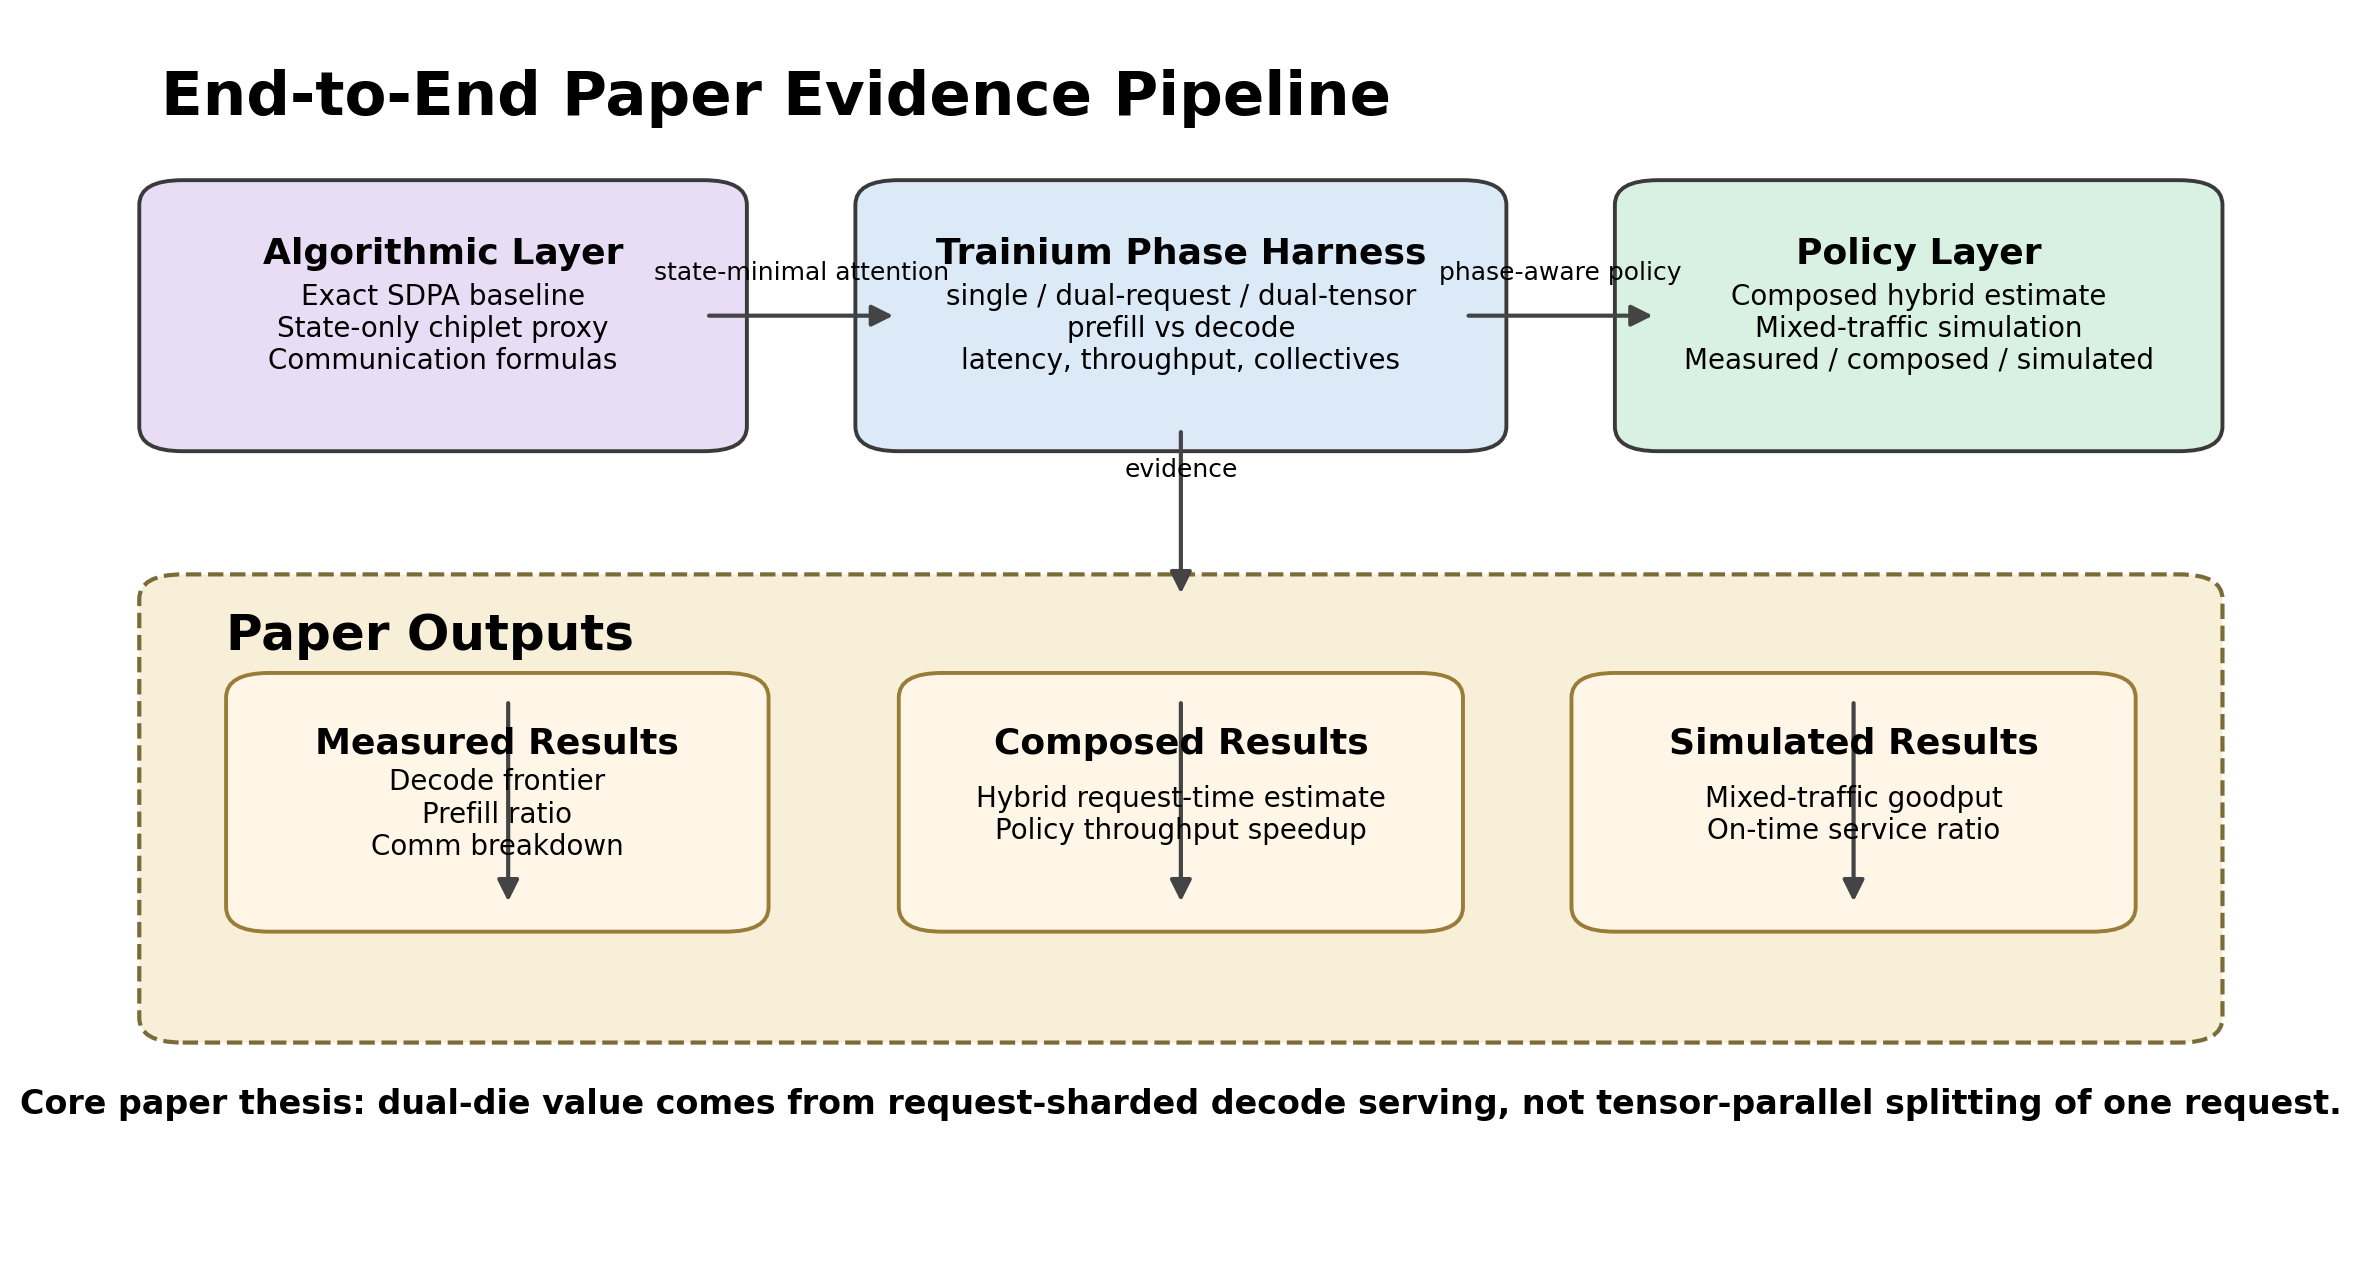
\includegraphics[width=\textwidth]{project_overview_pipeline.png}
  \caption{End-to-end evidence pipeline used in this paper package. The paper combines algorithmic evidence (state-only chiplet proxy), measured Trainium phase-study evidence, a measured direct policy trace, a composed policy estimate, and a simulated mixed-traffic evaluation.}
  \label{fig:overview-pipeline}
\end{figure*}

\section{Problem Statement}
We study attention execution strategies for non-GPU and multi-die accelerators under three constraints: limited local memory, explicit partition boundaries, and non-trivial cross-die collective cost. The target workload is forward-only scaled dot-product attention (SDPA). The task is to determine which partitioning strategy preserves correctness, reduces communication, and improves inference service performance.

\textbf{Algorithmic task.} Given $Q$, $K$, and $V$, execute exact SDPA while partitioning $K/V$ across two islands and exchanging only online-softmax state. The output must match monolithic SDPA within numerical tolerance.

\textbf{Systems task.} Given a Trainium-class dual-die serving substrate, decide whether dual-die should be used to (i) split one request's computation or (ii) distribute concurrent decode work across dies. The design target is not training throughput but inference service latency and throughput under realistic phase structure.

\textbf{Assumptions and constraints.}
\begin{itemize}[leftmargin=1.3em]
  \item The chiplet proxy uses two partitions, an even K/V split, full precision, and synchronous merge.
  \item Communication in the chiplet proxy is modeled by words exchanged; link latency is not simulated there.
  \item The Trainium artifact is compact rather than exhaustive: two prefill lengths and two decode concurrencies at context 2048.
  \item We include both a direct end-to-end policy trace and a composed per-phase estimate; the composed view is used for attribution and decomposition.
  \item Mixed-traffic figures are simulations driven by measured phase profiles.
\end{itemize}

\section{Methodology and Implementation}
\subsection{Algorithmic chiplet proxy}
The chiplet proxy is based on online softmax. For each query row, each partition computes a local running max $m_i$, normalizer $l_i$, and partial output vector $o_i$. The global result is merged using the standard online-softmax recurrence:
\begin{equation}
  m = \max(m_0, m_1),
\end{equation}
\begin{equation}
  l = e^{m_0-m} l_0 + e^{m_1-m} l_1,
\end{equation}
\begin{equation}
  o = \frac{e^{m_0-m} l_0 o_0 + e^{m_1-m} l_1 o_1}{l}.
\end{equation}
This formulation is exact up to floating-point tolerance and crosses the partition boundary with state rather than materialized scores. The key consequence is communication complexity. State-only exchange scales as $O(S(2 + D_v))$, whereas score+value exchange scales as $O(S^2(1 + D_v))$.

\subsection{Trainium phase harness}
The systems harness compares three execution modes:
\begin{itemize}[leftmargin=1.3em]
  \item \texttt{single\_die}: monolithic baseline;
  \item \texttt{dual\_die\_request\_sharded}: concurrent decode requests or KV footprint distributed across dies; and
  \item \texttt{dual\_die\_tensor\_optimized}: tensor-split execution of a single request.
\end{itemize}
Prefill and decode are benchmarked separately. The harness records p50/p90 latency, tokens/s throughput, compute time, communication time, and collective breakdowns. These measurements feed three downstream policy analyses:
\begin{itemize}[leftmargin=1.3em]
  \item a \textbf{measured} direct end-to-end policy trace over full request lifecycles;
  \item a \textbf{composed} hybrid-policy estimator that combines measured prefill cost with measured decode throughput; and
  \item a \textbf{simulated} mixed-traffic evaluation driven by measured phase profiles.
\end{itemize}

\subsection{Evidence typing}
The paper uses three evidence types and labels them explicitly:
\begin{itemize}[leftmargin=1.3em]
  \item \textbf{Measured}: decode frontier, prefill ratio, attention communication breakdown, and direct end-to-end policy trace.
  \item \textbf{Composed}: phase-aware hybrid request-time estimate.
  \item \textbf{Simulated}: mixed-traffic goodput under a synthetic request stream.
\end{itemize}
This separation is important because the best paper story comes from integrating these evidence layers without pretending they are all the same kind of experiment.

\section{Experimental Setup}
\subsection{Chiplet proxy}
The algorithmic chiplet proxy uses fixed random seeds, float32 arithmetic, and evenly partitioned K/V tensors. The example configuration used in the paper package is $S=16$, $D=8$, $D_v=8$, seed $7$. The outputs reported are max absolute error against monolithic SDPA and analytical communication counts for state-only, score-only, and score+value exchange.

\subsection{Trainium phase study}
The committed phase artifact evaluates prefill at sequence lengths 2048 and 4096 and decode at context length 2048 with concurrency 8 and 16. Metrics include p50 and p90 latency, tokens/s throughput, and compute/communication breakdown. We additionally run a direct end-to-end policy trace at context length 2048, output length 128, batch/concurrency 16, and a 1500\,ms request SLO for three policies: single$\rightarrow$single, single$\rightarrow$request, and request$\rightarrow$request. The mixed-traffic simulator uses a 90\,s synthetic trace with arrival rate 10 requests/s, 30\% prefill traffic, and a 250\,ms decode SLO.

\subsection{Comparison baselines}
For the chiplet proxy, the baseline is monolithic exact SDPA; communication comparisons are analytical score-only and score+value exchange. For the Trainium study, \texttt{single\_die} is the baseline against both dual-die strategies. For MoE, the baseline is single-die for absolute performance and dual-naive for locality-aware routing gain.

\section{Evaluation}
\begin{table*}[t]
  \centering
  \caption{Headline results from committed artifacts. Phase results are measured on Trn2. Mixed-traffic results are simulated from measured phase profiles. Ratios are relative to the baseline in the same block.}
  \label{tab:headline}
  \footnotesize
  \begin{minipage}{0.62\textwidth}
    \centering
    \begin{tabular}{lcccc}
      \toprule
      Phase & Metric & Single & Dual-request & Dual-tensor \\
      \midrule
      Decode (ctx=2048, C=16) & tok/s & 1212.5 & 1571.6 (\textbf{1.30}$\times$) & 347.4 (\textbf{0.29}$\times$) \\
      & p50 ms & 52.8 & 40.7 (\textbf{0.77}$\times$) & 184.2 (\textbf{3.49}$\times$) \\
      Decode (ctx=2048, C=8) & tok/s & 657.0 & 736.9 (1.12$\times$) & 184.3 (\textbf{0.28}$\times$) \\
      & p50 ms & 48.7 & 43.4 (0.89$\times$) & 173.6 (\textbf{3.57}$\times$) \\
      Prefill (S=4096, B=2) & p50 ms & 36.7 & 40.6 (1.11$\times$) & 1646.1 (\textbf{44.8}$\times$) \\
      \bottomrule
    \end{tabular}
  \end{minipage}
  \hfill
  \begin{minipage}{0.36\textwidth}
    \centering
    \begin{tabular}{lcccc}
      \toprule
      Policy (sim) & Goodput tok/s & vs single & On-time & p90 ms \\
      \midrule
      single$\rightarrow$single & 8172 & 1.00$\times$ & 57.6\% & 526.2 \\
      single$\rightarrow$request & 11304 & \textbf{1.38}$\times$ & \textbf{91.4}\% & 235.6 \\
      request$\rightarrow$request & 11277 & 1.38$\times$ & 90.9\% & 241.7 \\
      single$\rightarrow$tensor & 159 & \textbf{0.02}$\times$ & 1.2\% & 2346.4 \\
      \bottomrule
    \end{tabular}
  \end{minipage}
\end{table*}

\subsection{State-only exchange is exact and asymptotically communication-efficient}
Table~\ref{tab:chiplet-example} shows the chiplet-proxy example. The merge is numerically exact to floating-point tolerance. At this tiny shape, state-only exchange is slightly larger than score-only exchange because the state vector contains $2 + D_v = 10$ scalars per partition per query. But the more relevant comparison is against score+value exchange, where state-only is already \num{7.2}$\times$ smaller. Figure~\ref{fig:chiplet-scaling} shows the asymptotic picture: as sequence length grows, state-only exchange grows linearly while score and score+value exchange grow quadratically.

\begin{table}[t]
  \centering
  \caption{Chiplet-proxy example used in the paper package.}
  \label{tab:chiplet-example}
  \begin{tabular}{lrr}
    \toprule
    Metric / scheme & Value & Relative to state \\
    \midrule
    max $\lvert y_{\text{base}} - y_{\text{proxy}} \rvert$ & \num{2.082e-17} & -- \\
    state-only exchange & 320 words & \num{1.00}$\times$ \\
    score-only exchange & 256 words & \num{0.80}$\times$ \\
    score+value exchange & 2304 words & \num{7.20}$\times$ \\
    correctness & PASS & -- \\
    \bottomrule
  \end{tabular}
\end{table}

\begin{figure}[t]
  \centering
  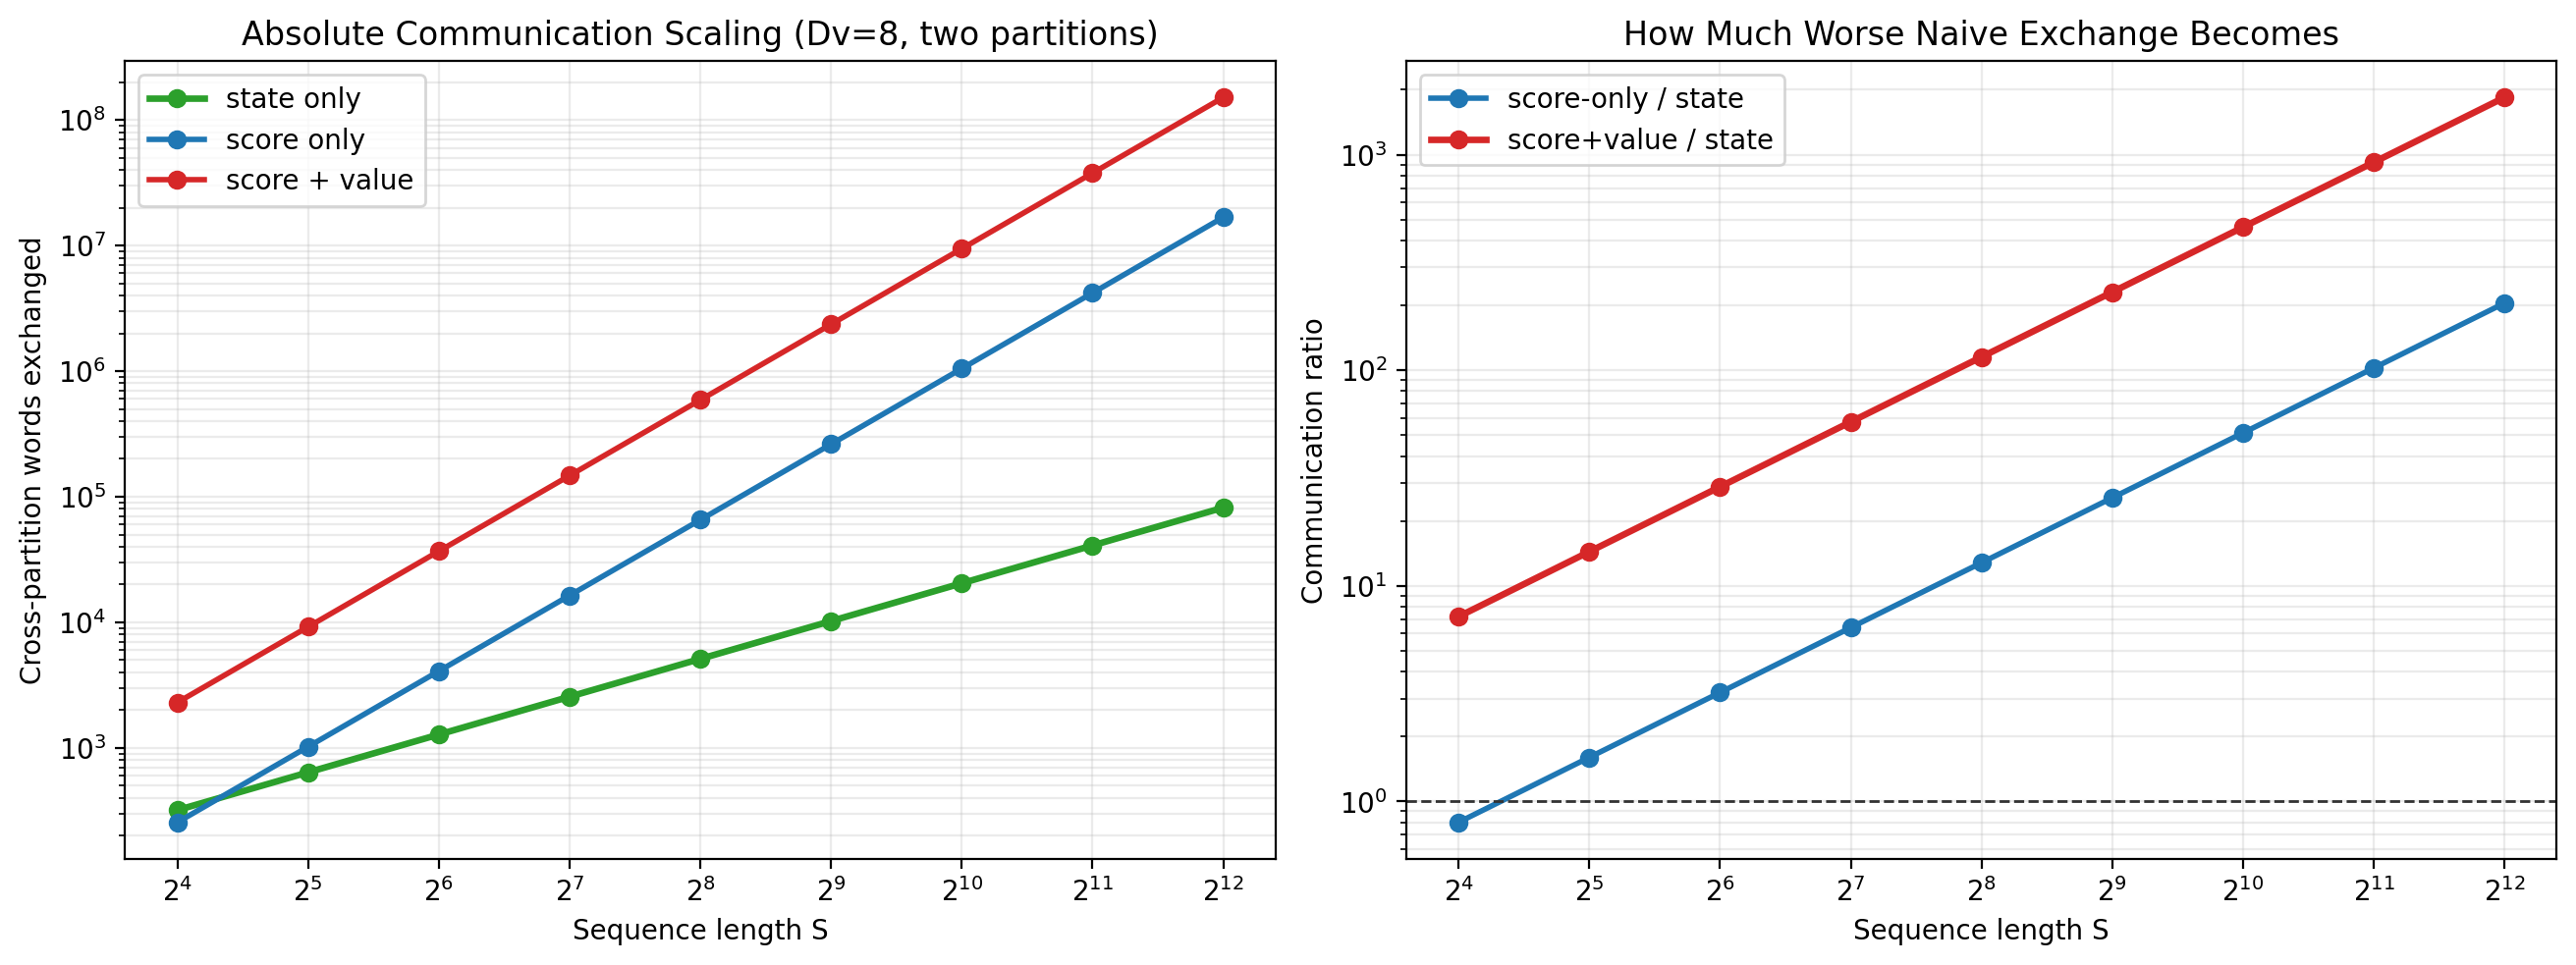
\includegraphics[width=\columnwidth]{chiplet_comm_scaling.png}
  \caption{Analytical communication scaling for two-partition attention with $D_v=8$. State-only exchange grows linearly with sequence length, while naive score and score+value exchange grow quadratically.}
  \label{fig:chiplet-scaling}
\end{figure}

\subsection{Request-sharded dual-die decode wins; tensor-split decode loses}
The central measured result is shown in Figure~\ref{fig:decode-frontier} and Table~\ref{tab:decode-summary}. At context length 2048, request-sharded dual-die improves both decode points in the committed artifact. At concurrency 16, throughput rises from \num{1212.5} to \num{1571.6} tokens/s (\num{1.30}$\times$) and p50 latency drops from \num{52.8} to \num{40.7}\,ms (\num{0.77}$\times$). Tensor-split dual-die does the opposite, dropping to \num{347.4} tokens/s (\num{0.29}$\times$ of single-die throughput) and rising to \num{184.2}\,ms p50 latency (\num{3.49}$\times$ slower).

\begin{figure}[t]
  \centering
  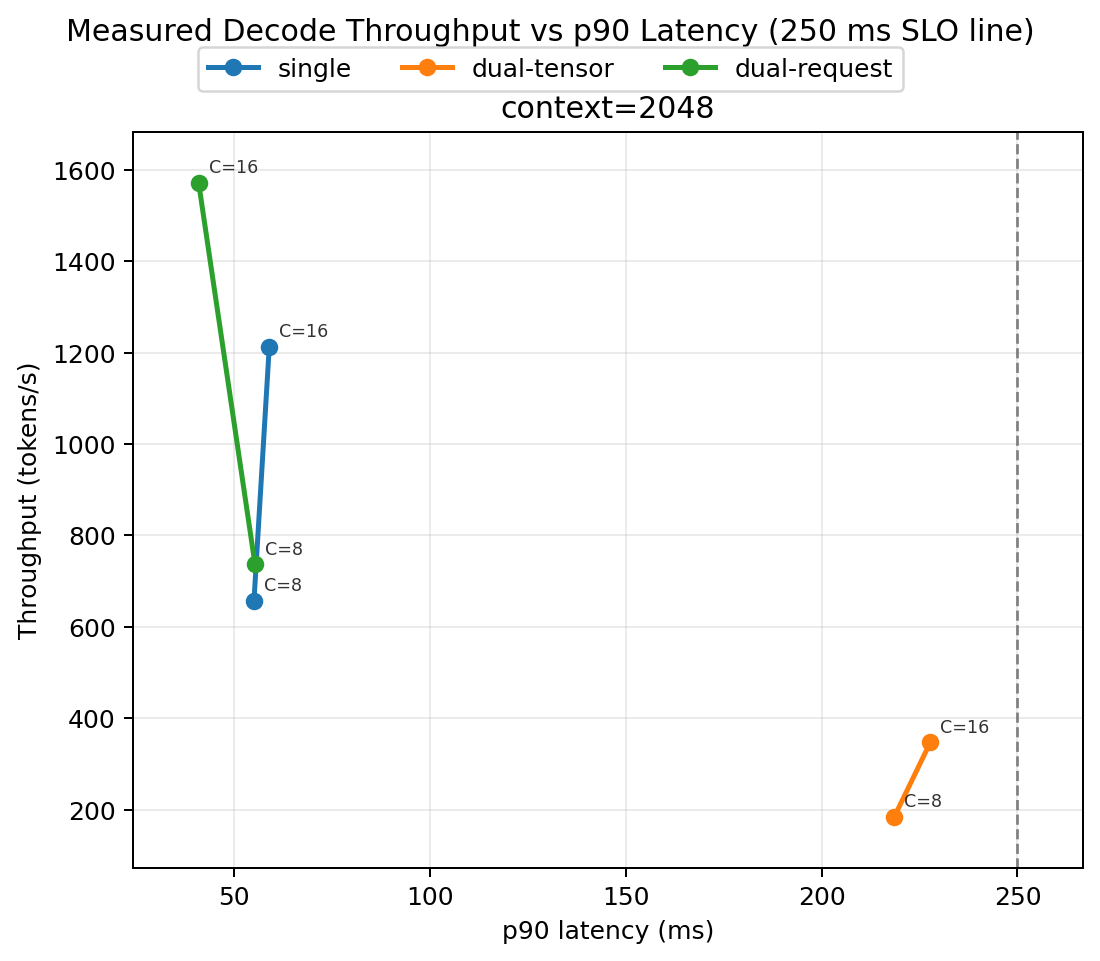
\includegraphics[width=\columnwidth]{public_service_decode_slo_frontier.png}
  \caption{Measured decode throughput versus p90 latency. Request-sharded dual-die is the only dual-die path that moves the frontier in the right direction.}
  \label{fig:decode-frontier}
\end{figure}

\begin{table}[t]
  \centering
  \caption{Measured decode summary at context length 2048.}
  \label{tab:decode-summary}
  \begin{tabular}{lrrrr}
    \toprule
    Setup & C=8 p50 & C=8 tok/s & C=16 p50 & C=16 tok/s \\
    \midrule
    single-die & 48.7 & 657.0 & 52.8 & 1212.5 \\
    dual-request & 43.4 & 736.9 & 40.7 & 1571.6 \\
    dual-tensor & 173.6 & 184.3 & 184.2 & 347.4 \\
    \bottomrule
  \end{tabular}
\end{table}

\subsection{Low-batch long-context prefill still prefers single-die}
Dual-die does not help all phases. In the committed low-batch prefill point (sequence length 4096, batch 2), request-sharded dual-die is \num{1.11}$\times$ slower than single-die, while tensor-split dual-die is \num{44.8}$\times$ slower. That phase asymmetry is exactly why a static ``always dual-die'' story is incorrect.

\begin{figure}[t]
  \centering
  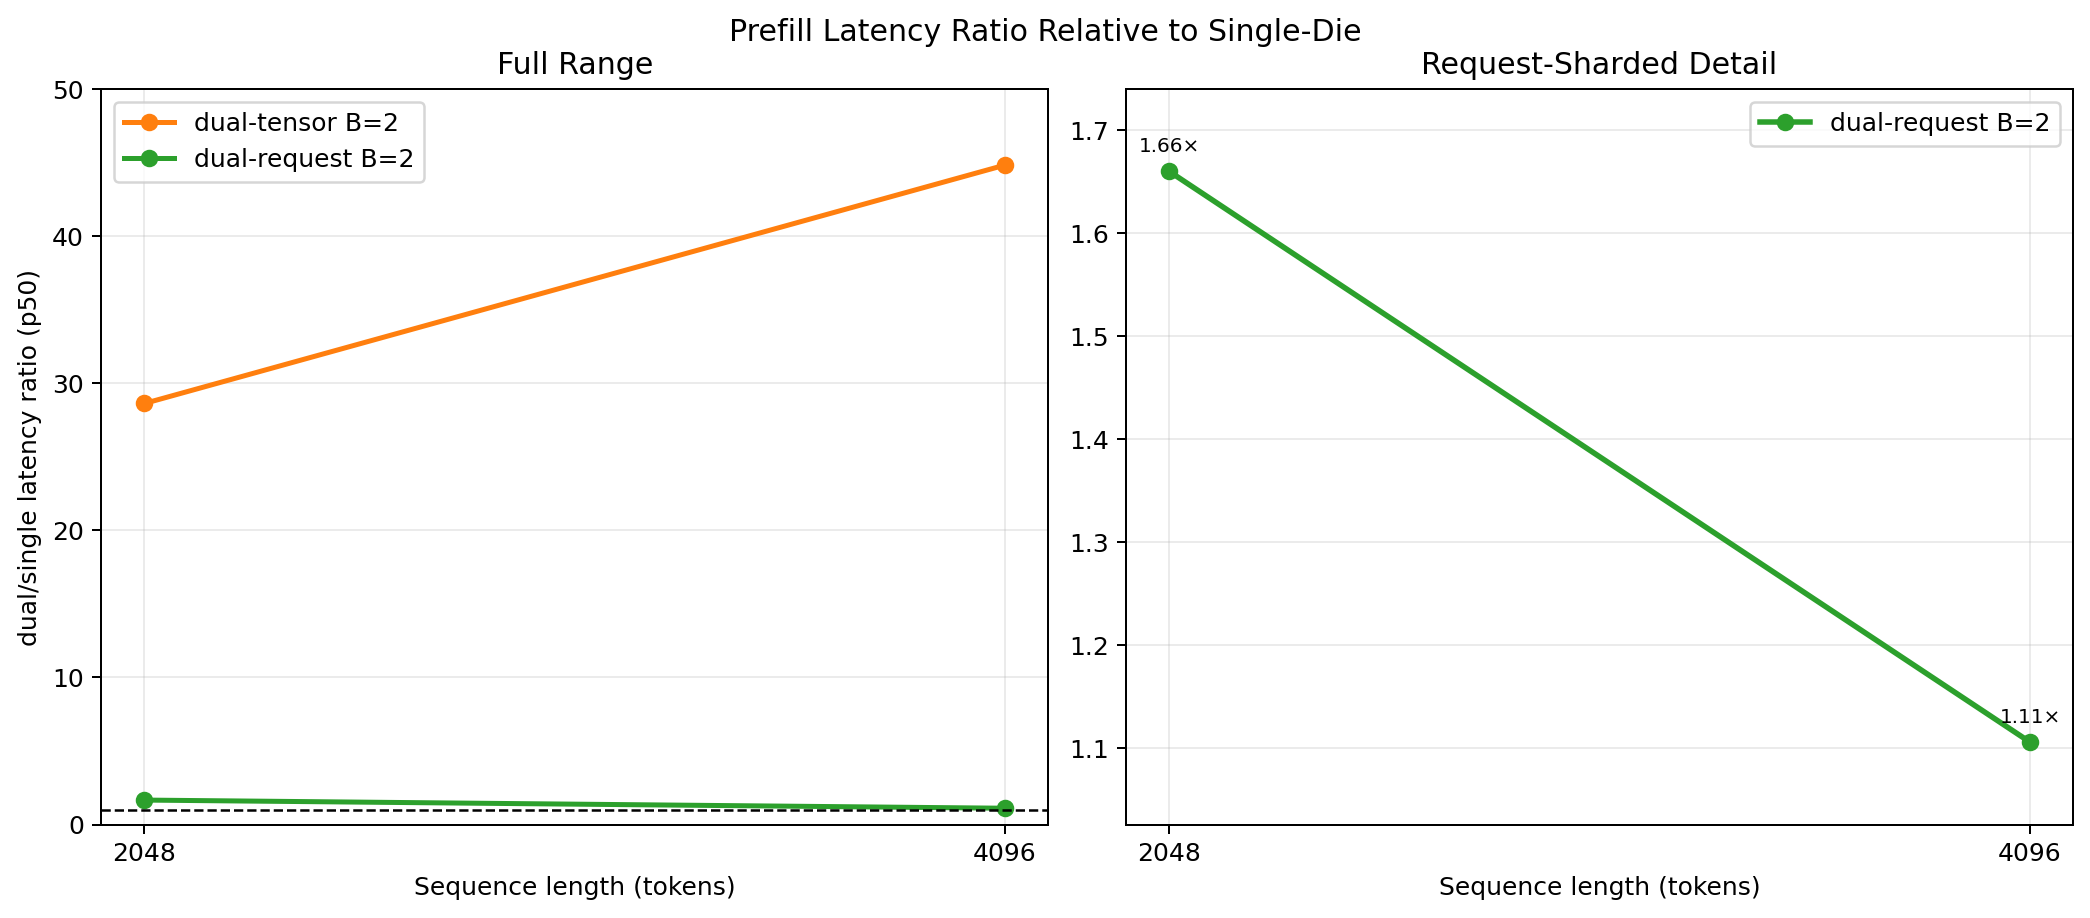
\includegraphics[width=\columnwidth]{public_service_prefill_ratio.png}
  \caption{Prefill latency ratio relative to single-die. Left: full range including the tensor-split collapse. Right: request-sharded detail, which makes the useful signal legible without hiding the larger 2048-point penalty.}
  \label{fig:prefill-ratio}
\end{figure}

\subsection{Why tensor splitting loses: communication structure, not just bytes}
Tensor-split decode fails for structural reasons. Figure~\ref{fig:comm-breakdown} shows a representative attention microbenchmark where the optimized dual path spends a large fraction of time in collectives. The supporting phase artifact is even more revealing: at prefill sequence length 4096, an \texttt{all\_reduce\_max} totaling only 4\,MB takes roughly 1245\,ms, while an \texttt{all\_gather} totaling 128\,MB takes only 9.7\,ms. The bottleneck is collective class and count, not only raw payload size.

\begin{figure}[t]
  \centering
  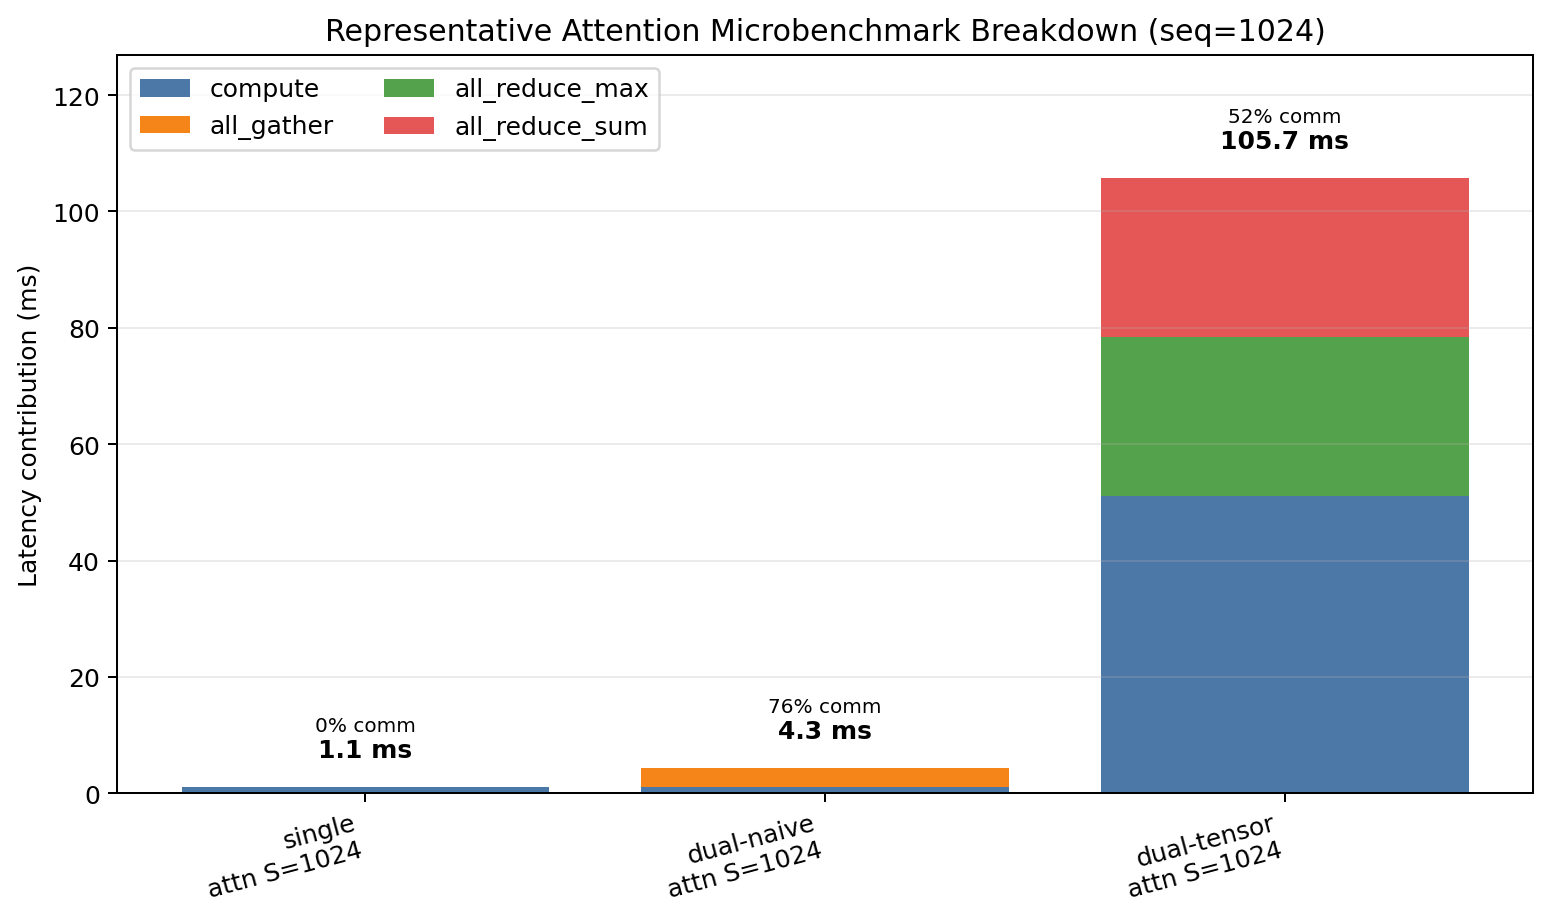
\includegraphics[width=\columnwidth]{public_service_comm_breakdown.png}
  \caption{Representative attention microbenchmark breakdown. The tensor-split dual path is dominated by collective operations, showing that synchronization structure---not only compute partitioning---drives the latency collapse.}
  \label{fig:comm-breakdown}
\end{figure}

\subsection{Direct trace: request-aware policies dominate end-to-end}
The highest-value validation is a direct measured end-to-end trace. Figure~\ref{fig:direct-trace} and Table~\ref{tab:direct-trace} report a full request lifecycle at context 2048, batch/concurrency 16, output tokens 128, and request SLO 1500\,ms. Relative to single$\rightarrow$single, both request-aware policies improve p50 requests/s by about \num{1.32}--\num{1.33}$\times$ and move on-time service from 0\% to 100\%. The two request-aware policies are close (\num{11.52} vs \num{11.62} req/s), which is expected because this point is decode-heavy and both policies use request-sharded decode.

\begin{figure}[t]
  \centering
  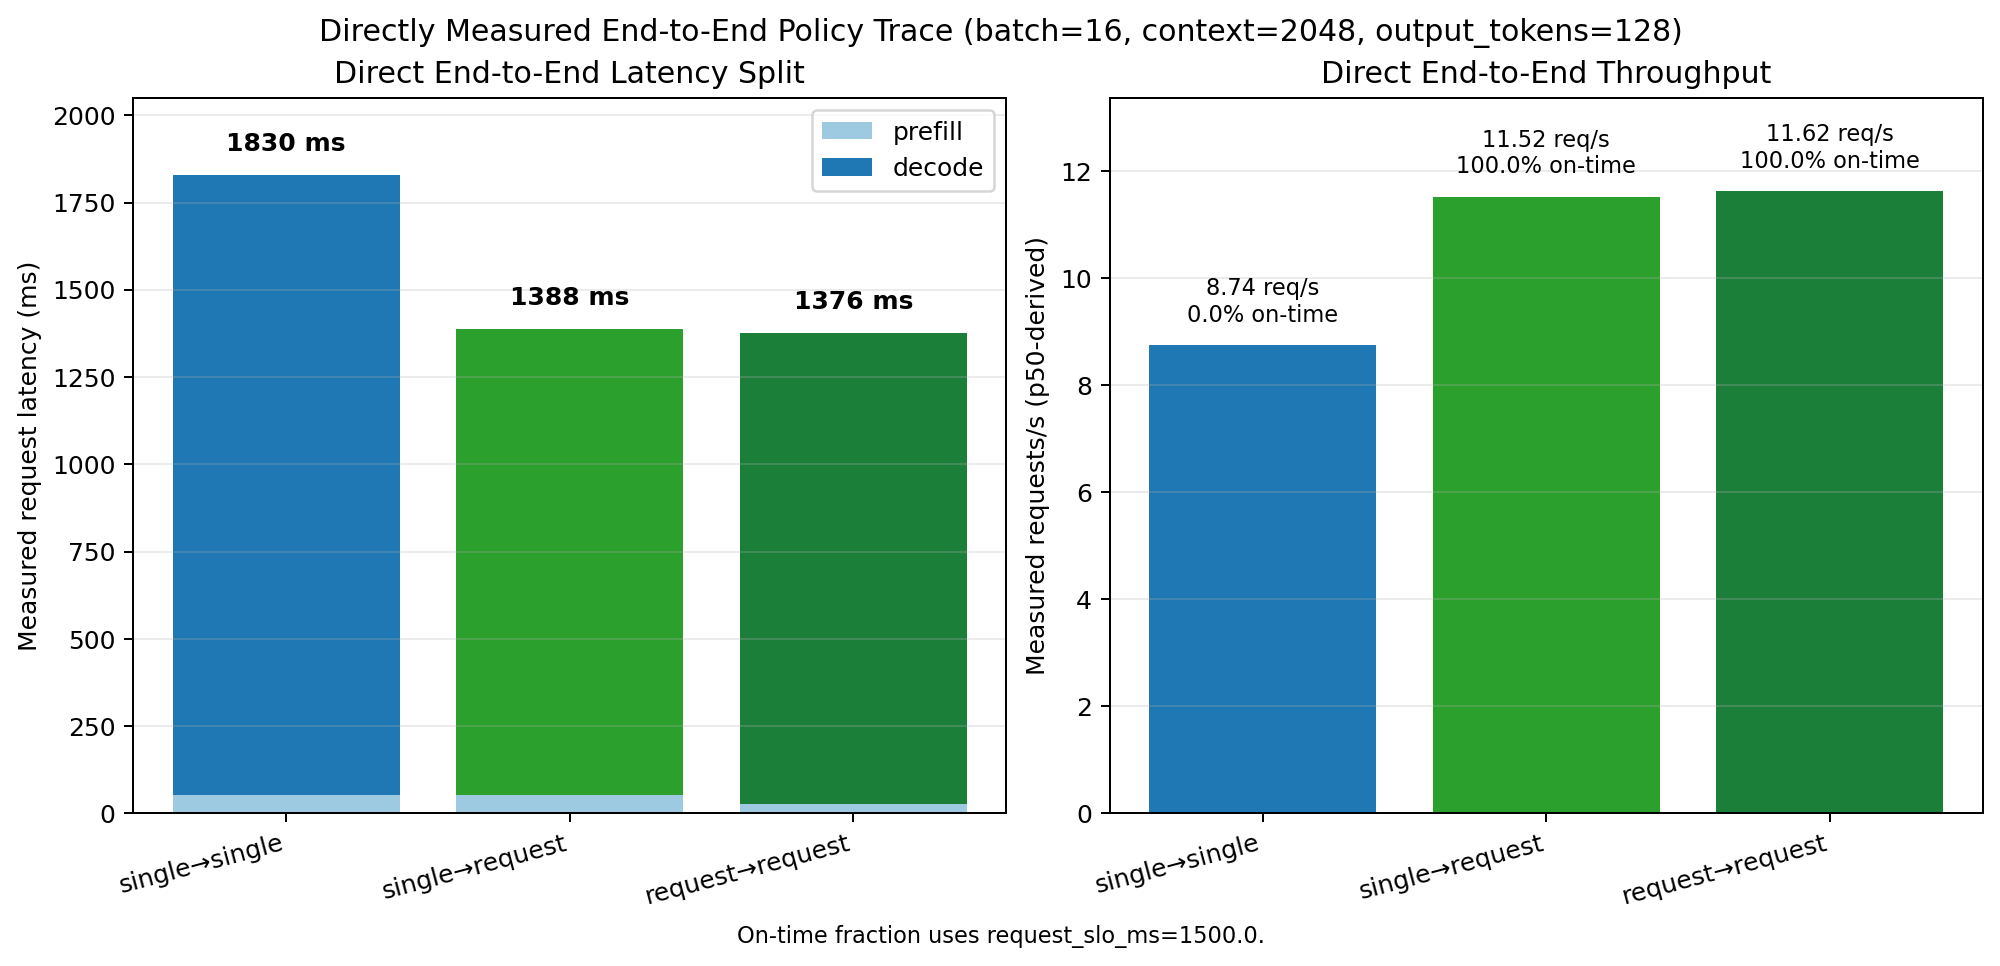
\includegraphics[width=\columnwidth]{public_service_direct_policy_trace.png}
  \caption{Directly measured end-to-end policy trace at context 2048, batch/concurrency 16, output tokens 128. Bars split prefill and decode p50 latency, and throughput is reported as p50-derived requests/s with on-time fraction under a 1500\,ms SLO.}
  \label{fig:direct-trace}
\end{figure}

\begin{table}[t]
  \centering
  \caption{Directly measured end-to-end policy trace summary.}
  \label{tab:direct-trace}
  \begin{tabular}{lrrrr}
    \toprule
    Policy & p50 ms & p90 ms & Req/s & On-time \% \\
    \midrule
    single$\rightarrow$single & 1830.1 & 1841.1 & 8.74 & 0.0 \\
    single$\rightarrow$request & 1388.5 & 1399.9 & 11.52 & 100.0 \\
    request$\rightarrow$request & 1376.5 & 1389.7 & 11.62 & 100.0 \\
    \bottomrule
  \end{tabular}
\end{table}

\subsection{Composed and simulated views broaden coverage}
Once prefill and decode are separated, composed and simulated policy tools remain useful for broader sweeps and attribution. Figure~\ref{fig:hybrid-estimate} composes measured prefill latency with measured decode throughput into a per-request estimate for 128 output tokens. In the committed phase artifact, single$\rightarrow$request is the strongest composed policy because it keeps the lower measured prefill cost of single-die while exploiting decode gains from request sharding.

\begin{figure}[t]
  \centering
  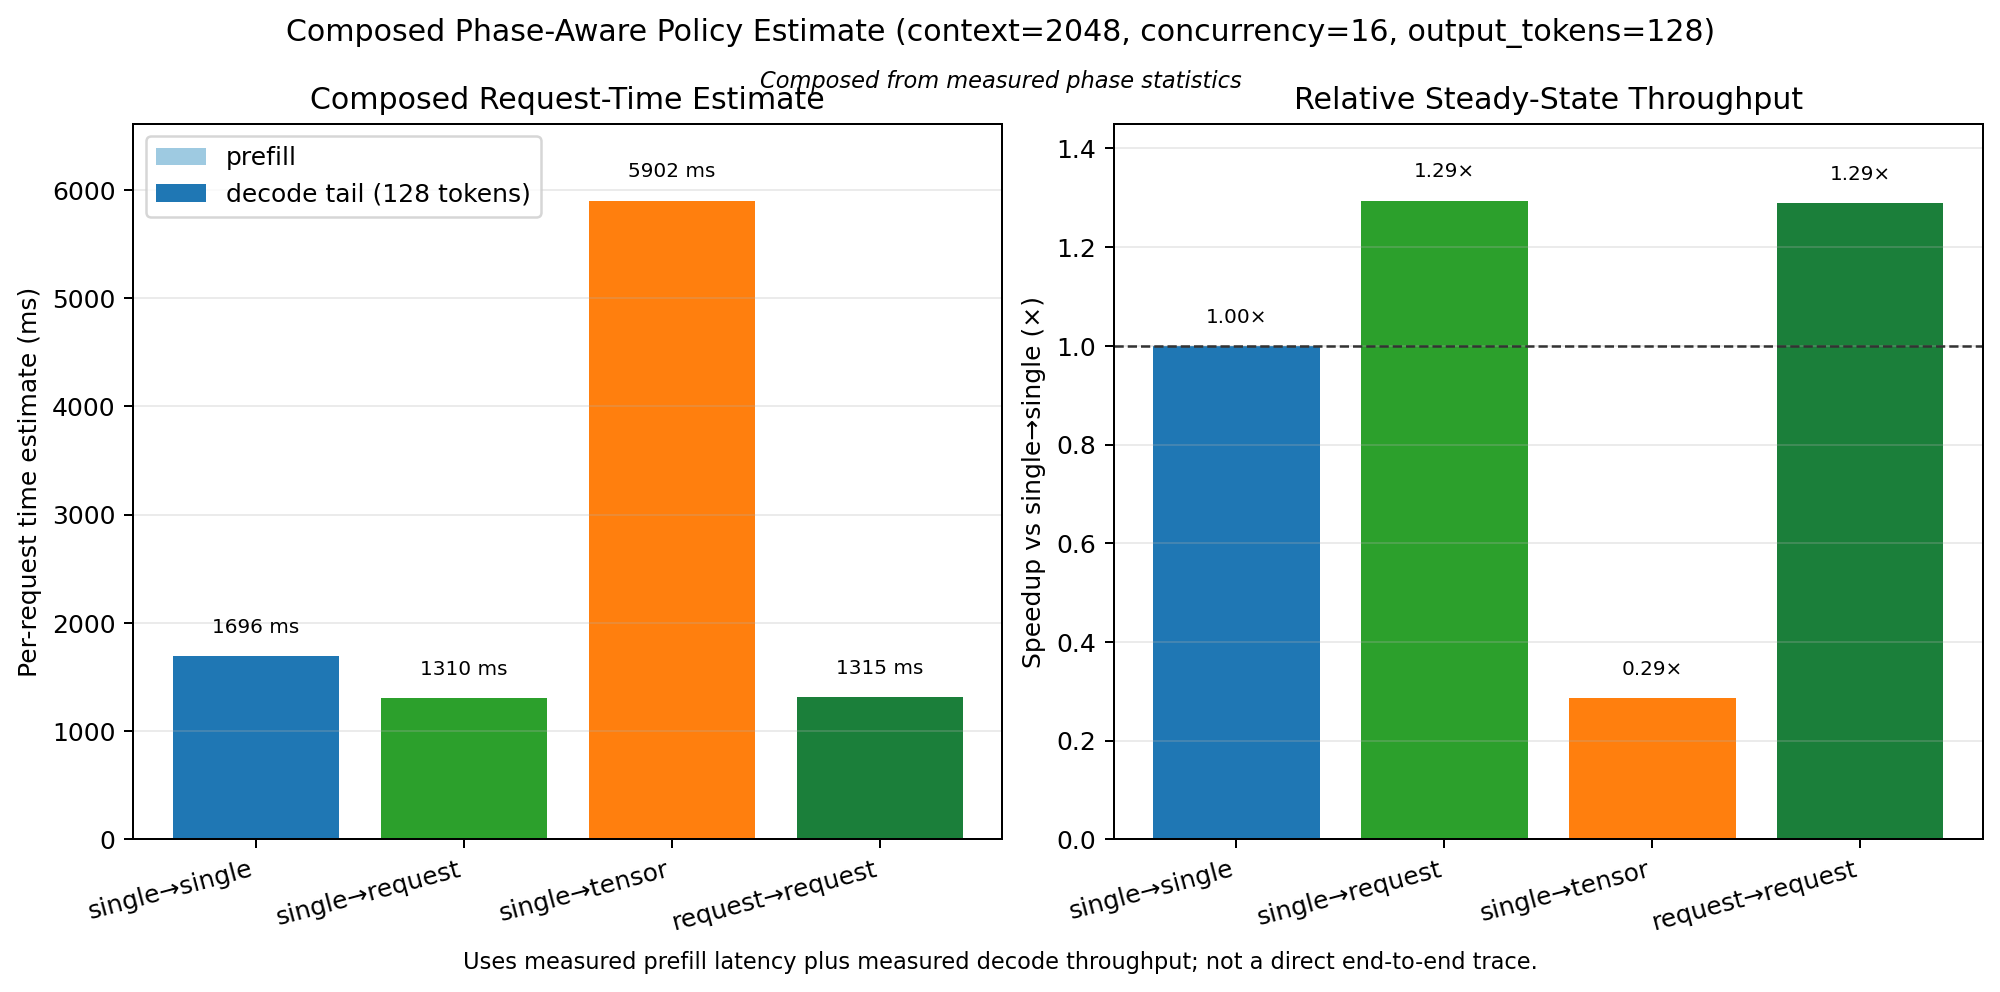
\includegraphics[width=\columnwidth]{public_service_hybrid_e2e.png}
  \caption{Composed phase-aware policy estimate from measured prefill latency and measured decode throughput. This plot is used to compare policy choices, not to replace a direct end-to-end serving trace.}
  \label{fig:hybrid-estimate}
\end{figure}

The mixed-traffic simulator reaches the same ordering. Table~\ref{tab:mixed-traffic} and Figure~\ref{fig:mixed-traffic} show that single$\rightarrow$request improves goodput from \num{8172} to \num{11304} tokens/s (\num{1.38}$\times$) and raises on-time service from 57.6\% to 91.4\%. Request$\rightarrow$request is nearly tied, while single$\rightarrow$tensor collapses.

\begin{table}[t]
  \centering
  \caption{Mixed-traffic policy comparison from the committed simulator trace.}
  \label{tab:mixed-traffic}
  \begin{tabular}{lrrr}
    \toprule
    Policy & Goodput tok/s & On-time \% & p90 ms \\
    \midrule
    single$\rightarrow$single & 8172.1 & 57.6 & 526.2 \\
    single$\rightarrow$request & 11303.8 & 91.4 & 235.6 \\
    request$\rightarrow$request & 11276.8 & 90.9 & 241.7 \\
    single$\rightarrow$tensor & 159.3 & 1.2 & 2346.4 \\
    \bottomrule
  \end{tabular}
\end{table}

\begin{figure}[t]
  \centering
  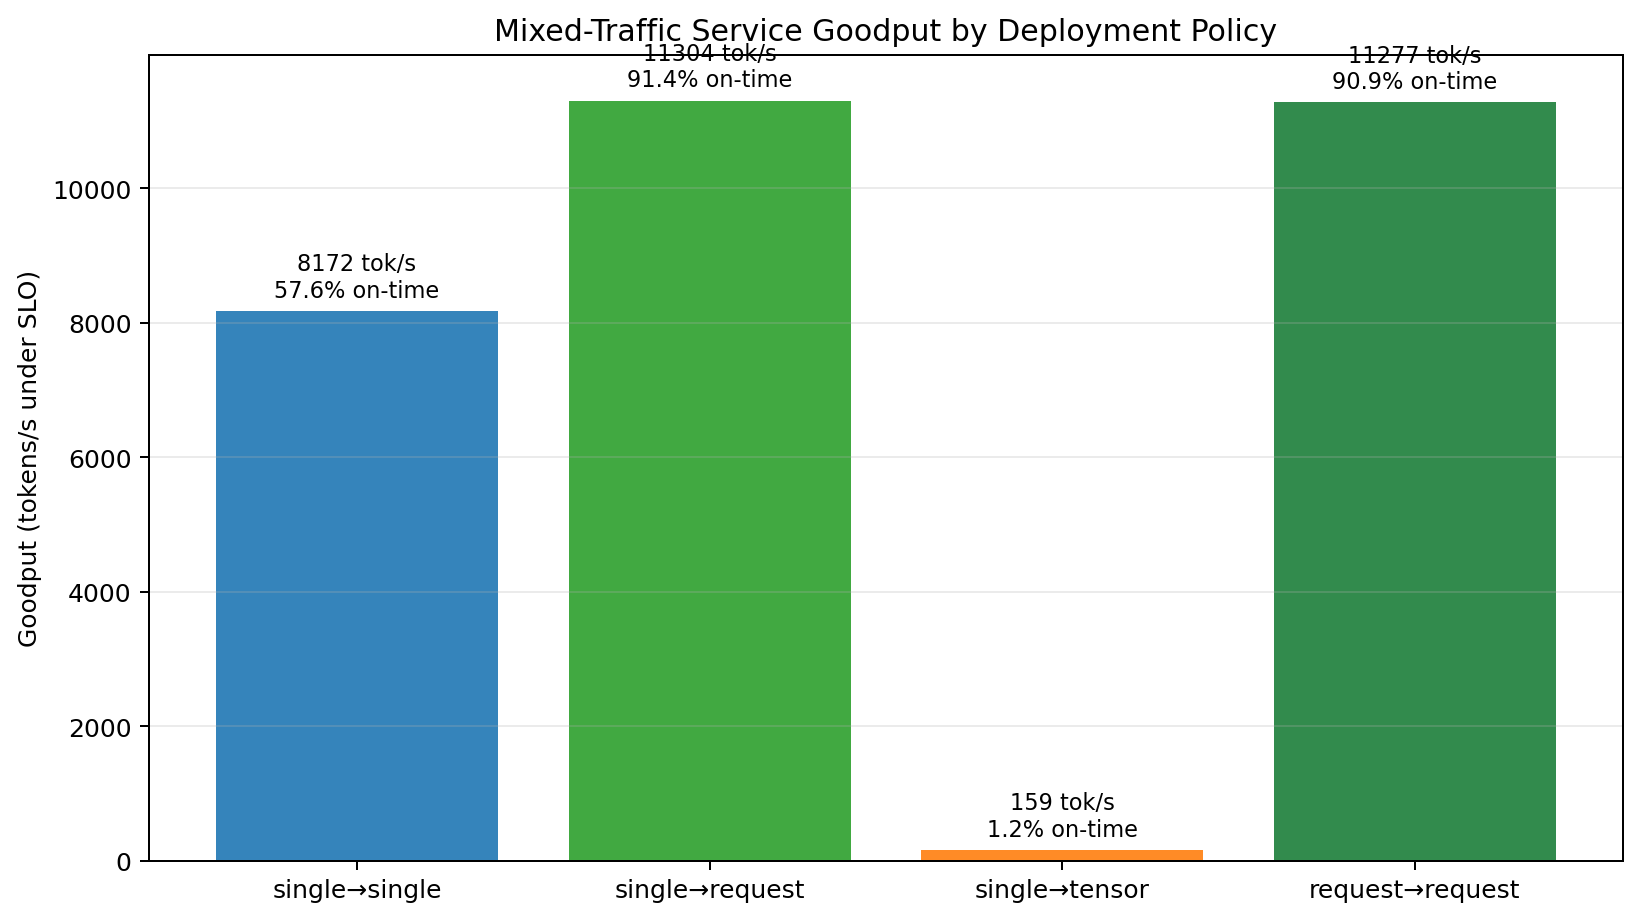
\includegraphics[width=\columnwidth]{public_service_mixed_trace_goodput.png}
  \caption{Simulated mixed-traffic goodput. The same ordering from the phase study reappears under queueing pressure: request-aware decode policies dominate, while tensor-split decode fails.}
  \label{fig:mixed-traffic}
\end{figure}

\subsection{Secondary evidence: MoE locality helps inside the dual path}
The MoE artifact is secondary evidence rather than the paper's headline. Single-die remains far faster in absolute throughput, so MoE does not overturn the main single-vs-dual conclusion. The useful signal is narrower: locality-aware routing improves the dual path over naive routing, with a median throughput gain of \num{1.03}$\times$ and a median remote-dispatch reduction of 0.1875 absolute fraction. This is consistent with the broader claim that communication structure matters, but it becomes a positive systems story only when paired with the right workload regime.

\section{Discussion and Limitations}
The project has three main strengths. First, the chiplet proxy gives a clean correctness story for state-only distributed attention. Second, the Trainium phase harness separates prefill from decode, which prevents overclaiming. Third, the figure package makes evidence provenance explicit by separating measured, composed, and simulated results.

The limitations are equally important:
\begin{itemize}[leftmargin=1.3em]
  \item the chiplet proxy is a two-partition analytical model rather than a latency-aware network simulation;
  \item the canonical phase artifact is compact and should eventually be refreshed with a larger sweep;
  \item the direct end-to-end trace currently covers one main operating point (context 2048, batch 16, output 128) and should be expanded;
  \item the mixed-traffic result is simulated; and
  \item decode collective attribution in the older committed phase artifact predates the fixed per-op aggregation, so the paper uses the kernel artifact for the mechanism figure.
\end{itemize}
These caveats limit generality, but they do not change the paper's central lesson: on Trainium-class accelerators, dual-die value is primarily a serving-policy result, not a tensor-parallel kernel result.

\section{Related Work}
Our work is closest in spirit to IO-aware exact attention kernels such as FlashAttention and its follow-on work \citep{dao2022flashattention,dao2023flashattention2}. The key difference is target architecture. Rather than asking how to maximize GPU efficiency, we ask which IO-aware principles transfer to non-GPU and multi-die accelerators. The use of online-softmax merge state follows the same mathematical insight as online normalization \citep{milakov2018online}, but the contribution here is systems-oriented: using that state as the partition interface and then relating it to phase-aware serving behavior.

\section{Conclusion}
This paper argues for a more precise interpretation of dual-die attention. The value of dual-die is not universal latency reduction from tensor splitting. The stronger and more defensible result is phase-aware serving:
\begin{itemize}[leftmargin=1.3em]
  \item exact state-only merge preserves SDPA semantics while reducing communication versus score+value exchange;
  \item request-sharded dual-die decode improves measured service throughput and latency;
  \item a direct measured end-to-end trace confirms that request-aware policies improve on-time service and request throughput under serving load;
  \item tensor-split dual-die is communication-bound and loses in the committed regimes; and
  \item policy ranking is workload-dependent, but request-aware decode is consistently the dominant ingredient.
\end{itemize}
That is the novel systems lesson supported by this artifact set.

\bibliographystyle{plainnat}
\bibliography{refs}

\end{document}
